\subsection{Database Design}
This section presents the database design for the Horse Racing Tournament Management System. The persistent data layer is implemented using Microsoft SQL Server to store relational entity information.

Figure \ref{fig:db_design} displays the physical database design schema. The interactive database schema is also available online and can be accessed directly at: \href{https://dbdiagram.io/d/6a4a35fb36d348d1206d2224}{dbdiagram.io - Horse Racing Tournament Management System}.

\begin{figure}[H]
    \centering
    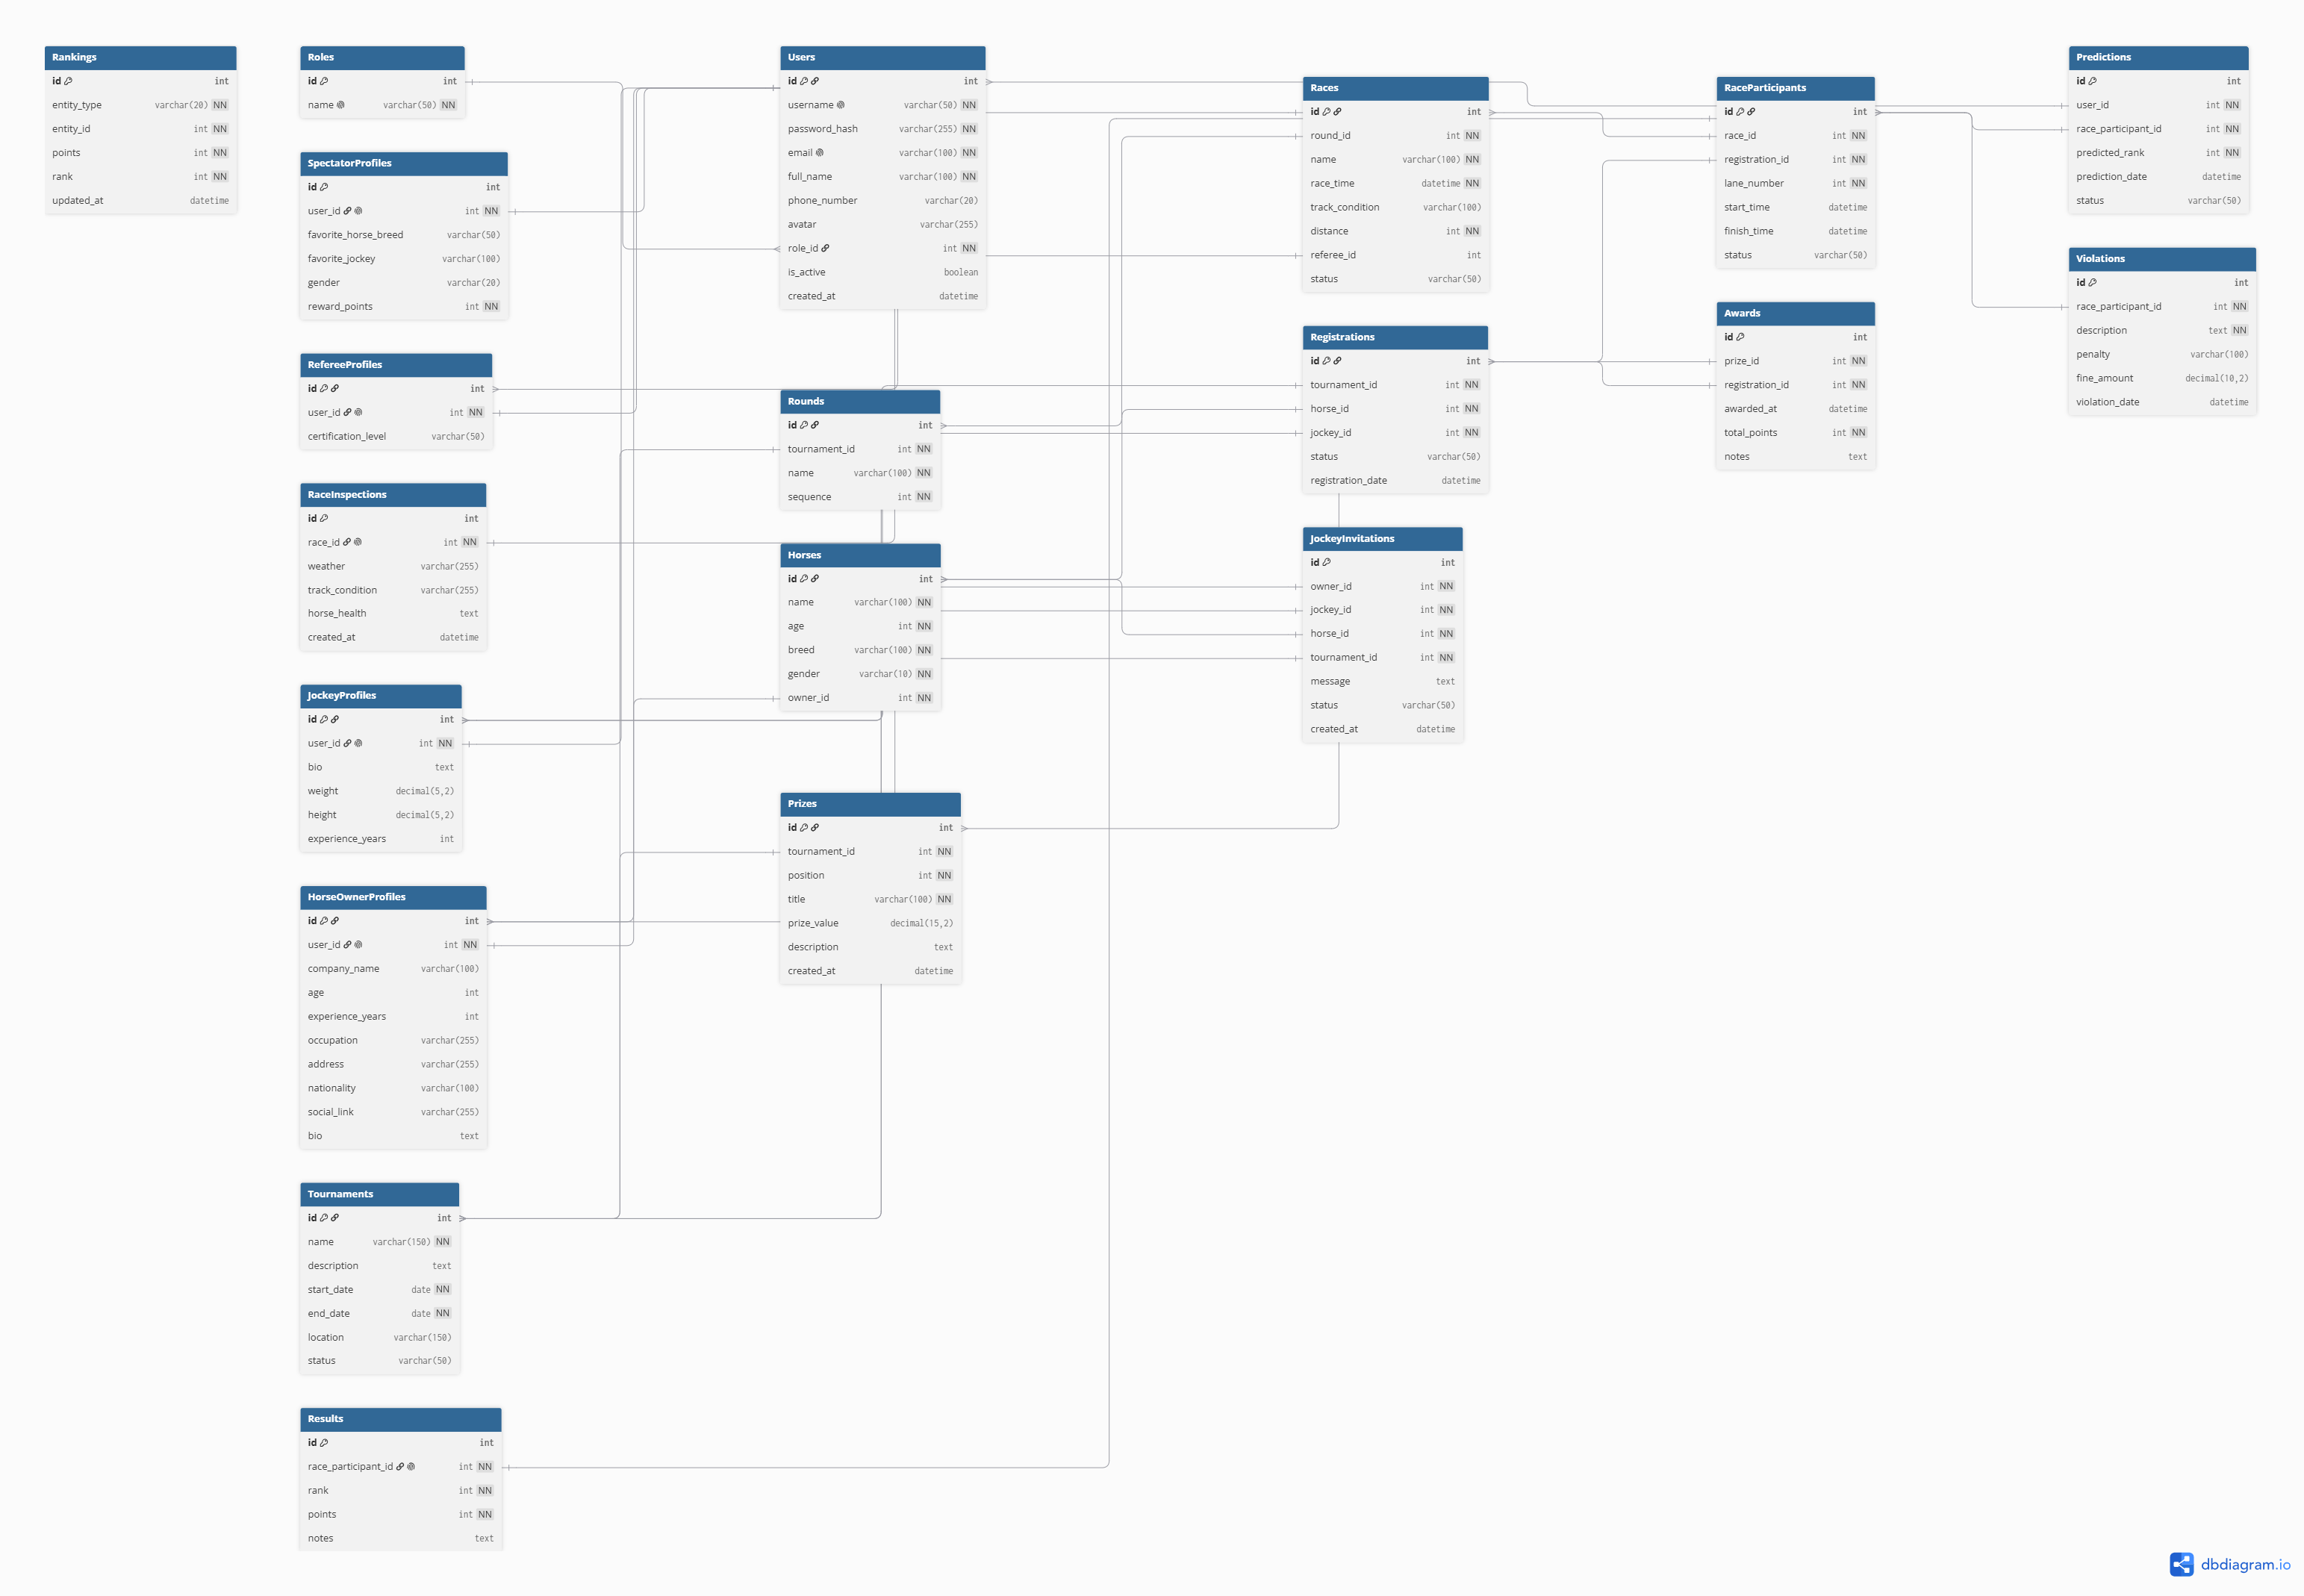
\includegraphics[width=0.95\textwidth]{figures/chuong4_diagram_chung/database_design.png}
    \caption{Physical Database Design Schema}
    \label{fig:db_design}
\end{figure}

The relational database schema is structured to capture all operations including user role-based access control, horse ownership details, tournament scheduling, race registration, and result calculation. Below is a detailed description of the physical table attributes:

\begin{itemize}
    \item \textbf{Roles:} Stores authorization group definitions (such as Admin, Referee, Jockey, Horse Owner, Spectator).
    \item \textbf{Users:} Holds centralized user profiles, password hashes, and links back to role definitions.
    \item \textbf{Profile Tables (JockeyProfiles, HorseOwnerProfiles, RefereeProfiles, SpectatorProfiles):} Extend the user table with domain-specific properties using 1-to-1 relationships.
    \item \textbf{Horses:} Tracks horse attributes and connects each horse to its respective owner profile.
    \item \textbf{Tournaments, Rounds, and Races:} Create a hierarchical structure representing active events, stages of competition, and individual races.
    \item \textbf{Registrations:} Acts as a junction table recording which horse and jockey pairings are approved to compete in a specific tournament.
    \item \textbf{RaceParticipants:} Manages lane allocations, race results (ranks/points), and violations for each registered participant in a specific race.
\end{itemize}
